This is an open source project under license GNU General Public License \cite{gplv3}. \\

\chapter{Introduction}

Sign or signed languages are complete natural languages that are expressed visually.
They have their own grammar, lexicon and are not universal. \\ 

Sign languages have became the main way of communicating between deaf-and-dumb people. Nevertheless,
it is not common in society to be able to understand them, so the gap between these communities
and the rest of society keeps increasing. \\

As a future Software Engineer, I have a big social responsability, because my developments and ideas
may help minorities and lessen gaps like this one. \\

Solutions such as a videocall application, that subtitles sign languages, could make sign language 
speakers be able to communicate with non-signers.
Although there are a lot of dictionaries and applications to learn sign language, there is an 
absence of applications that verify how you perform signing.
Learning sign language would be easier and more accessible if you would not need someone to do this verification,
and devices are now able to do this.

\section{Preliminar analysis. Viability study.}

In order to create an application to verify a signs or a videocall app, 
translating signs into text would be neccessary. \\

Previous works have their main focus on translating signs into text using special gloves. Although this is effective 
and would solve the problem, not everyone could afford these gloves imposing a barrier to entry. \\

The most accessible hardware for users would be the integrated cameras in their phones and pc's. Therefore,
the main objective of this initial study would be to analyse the efficiency and viability of translating 
a video into text using commodity hardware.

\subsection{Sign language characteristics}
The first thing that comes into mind is to develop a deep learning model able to translate signed sentences into 
text. Firstly, we should know the difficulties that this would take:
\begin{itemize}[noitemsep]
    \item In order to be able to translate a signed sentence into text, the model should understand the context to formulate the sentence correctly.
    \item Some words are signed the same way.
    \item Signs are performed differently if you are left-handed or right-handed.
    \item The dataset should contain videos of people from different ethnicities and sex signing.
\end{itemize}

Just analysing the alphabet would be a much simplier task, as all letters are signed statically (in ASL: American Sign Language), except the 'J' and 'Z'.
Therefore, a classification deep learning model could be developed to validate the images/videos from the user.
Nevertheless, such a system would be of little use and this functionality has already been developed and implemented by some applications such as Snapchat.

\subsection{Literature review}
This section contains a table with the main sources of information used in this work. \\

\begin{longtable}{|p{3cm}|p{4cm}|p{6cm}|}
    \hline {Type} & {Title} & {Note}      \\
    \hline Video & La INFRAESTRUCTURA detrás de TikTok \cite{TikTok2021} & Infraestructure analysis. How to divide a big service into smaller ones and create an UML diagram from it \\
    \hline Journal & Word-level Deep Sign Language Recognition from Video: A New Large-scale Dataset and Methods Comparison \cite{Li2019} & They introduce a large scale dataset for American Sign Language, consisting of 2000 words performed by more than 100 signers in more than 20.000 videos. They also introduce two models and compare them: holistic visual appearance-based approach, and 2D human pose based approach \\
    \hline Journal & Recognition of user-dependent and independent static hand gestures: Application to sign language \cite{Sadeddine2021} & Sign recognition becomes a very complex tax due to heterogeneous environment. This article studies how to improve accuracy of models using static hand gesture recognition based on a set of image descriptors: Gradient Local Auto-Correlation (GLAC), Gabor Wavelet Transform (GWT), and Fast Discrete Curve Transform (FDCT) \\
    \hline Journal & Optimization of convolutional neural networks architectures using pso for sign language recognition \cite{Fregoso2021} & It presents an approach to design convolutional neural network architectures, using the particle swarm optimization algorithm\\
    \hline Repository & TSPNet: Hierarchical Feature Learning via Temporal Semantic Pyramid for Sign Language Translation \cite{SLTTSPNet} & The repository contains the implementation of a deep learning model to translate from videos to text \\
    \hline Journal & Visual Alignment Constraint for Continuous Sign Language Recognition \cite{Min2021} & Work on how to solve the overfitting problem in recent CTC-based CSLR worksdue to the insufficient training of the feature extractor using a Visual Alignment Constraint (VAC) to enhance the feature extractor with more alignment supervision. It includes a code repository \\
    \hline Journal & ELM based two-handed dynamic Turkish Sign Language (TSL) word recognition \cite{ELM2021} & It studies the recognition of dynamic words in Turkish Sign Language (TSL) with two hands using the Leap Motion Controller (LMC) device \\
    \hline Journal & Applying deep neural networks for the automatic recognition of sign language words: A communication aid to deaf agriculturists \cite{Venugopalan2021} & In order to help deaf agriculturists, they propose a model using a LSTM trained using a small dataset of the most common indian signed-words in this field \\
    \hline Journal & Real-Time Sign Language Detection using Human Pose Estimation \cite{Moryossef2020} & Lightweight real-time sign language detection model for future use in videocall applications \\
    \hline Report  & Sign Language Transformers: Joint End-to-end Sign Language Recognition and Translation \cite{SignLanguageTransformers} & New architecture for continuous sign language recognition \\
    \hline Journal & Sign Language Recognition Using ConvolutionalNeural Networks \cite{Bronstein2015} & Recognition system using the Microsoft Kinect, convolutional neural networks (CNNs) and GPU acceleration \\
    \hline Video   & Real-Time Sign Language Detection for Video Conferencing Applications \cite{RT2021} & System for setting the main signer in a videoconferencing application \\
    \hline Website & American Sign Language Recognition in Python using Deep Learning \cite{ASLRecognitionPython} & Model that uses knowledge transfer to recognise letters in ASL \\
    \hline Website & How to use transfer learning for sign language recognition \cite{Vagdevi2019} & ResNet based model that uses knowledge transfer \\ 
    \hline Website & How to build a convolutional neural network that recognizes sign language gestures \cite{Vagdevi2019i} & Neural network to recognise letters in ASL \\
    \hline Journal & Sign Language Recognition for Computer Vision Enthusiasts \cite{Vaishshells2021} & Two models to recognise letters. A static one and a dynamic one using an american sign language dataset \\
    \hline Journal & ASL Alphabet \cite{Akash2018} & Dataset to sign letters in ASL. It transforms letters 'J' and 'Z' into images because they are signed dynamically (using movement) and requires video recognition. This way, the problem is reduced to an image classification one \\
    \hline Website & Hands-On Guide To Sign Language Classification Using CNN \cite{SignLanguageClassification2020} & Model to classify letters in ASL. It just classify static letters (all except 'J' and 'Z') \\
    \hline Journal & Sign Language Recognition: A Deep Survey \cite{Rastgoo2021} & State of art summary. It contains links to main models, datasets and architectures \\
    \hline Video   & Sign Language Detection using ACTION RECOGNITION with Python | LSTM Deep Learning Model \cite{SignLanguageRecognitionUsingActionRecognition} & Classify some ASL signs from a webcam \\
    \hline Video   & Real Time Sign Language Detection with Tensorflow Object Detection and Python | Deep Learning SSD \cite{SignLanguageRecognitionUsingObjectDetection} & App to recognise 5 static signs. It teaches how to create a dataset, label images and train a model from a dataset \\
    \hline Video   & Building a Real Time Sign Language Detection App with React.JS and Tensorflow.JS | Deep Learning \cite{SignLanguageRecognitionUsingReactjsAndTensorflow} & Shows how to transform a python model to a tensorflow one,upload it to the cloud and download it on the frontend, so that we can use it using a React.js app to validate videos on the client \\
    \hline Journal & Deep Learning Techniques for Spanish Sign Language Interpretation \cite{SpanishDataset2021} & Dataset for Spanish Sign Language recognition. It proposes to use CNNs to classify static letters and RNNs to classify dynamic letters \\
    \hline
    \caption{Literature review}
    \label{table:introduction_literature_review}
\end{longtable}

\subsection{Choosing a solution}
After carefully considering the literature review, my skills and the development time restrictions, I decided to create an application to learn American Sign Language. \\

The reasons that support this decision are:

\begin{itemize}[noitemsep]
    \item Availability of pretrained deep learning models that translate videos of people signing into text.
    \item Attainability of a medium-scale of a real-world dataset (American Sign Language \cite{Li2019}).
    \item Adecuate complexity level. The system is not as simple as the ones that only recognise individual letters and is not limited by a very small dataset.
\end{itemize}

\subsubsection{WLASL in depth: A large-scale dataset for Word-Level American Sign Language}
The WLASL was created due to the importance of American Sign Language for the deaf community, and the lack of a large-scale dataset that allows recognition at a word-level and a sentence-level.
It was chosen for this project due to its size and real-world recording conditions.

\paragraph{Characteristics}
The main characteristics of this dataset are:
\begin{itemize}[noitemsep]
    \item It is composed only by \textbf{monocular-RGB} videos: the videos do not rely on special equipment, such as depth cameras, colored gloves...
    \item All signers are in near-frontal views.
    \item The dataset contains 21.083 videos.
    \item Each video contains one sign in ASL.
    \item The videos are performed by 119 signers.
    \item Each sign is performed by at least 3 different signers.
    \item The average is 2.41 seconds (from 0.36 to 8.12 seconds).
\end{itemize}

\paragraph{Dataset structure}
The dataset is divided into four parts.
\begin{table}[h]
    \centering
    \resizebox{\textwidth}{!}{
    \begin{tabular}{|c|c|c|c|c|c|}
        \cline{1-6}  Datasets   & Gloss &  Videos &  Mean  & Signers   & Year       \\
        \hline       WLASL100   &   100 &   2,038 &  20.4  &      97   & 2019       \\
        \hline       WLASL300   &   300 &   5,117 &  17.1  &     109   & 2019       \\
        \hline      WLASL1000   &  1000 &  13,168 &  13.2  &     116   & 2019       \\
        \hline      WLASL2000   &  2000 &  21,083 &  10.5  &     119   & 2019       \\
        \hline
    \end{tabular}
    }
\caption{WLASL dataset structure}
\label{table:introduction_dataset_subdivisions}
\end{table}

\paragraph{Models proposed} The paper associated to the WLASL dataset proposes two models:
\begin{itemize}[noitemsep]
    \item I3D: it follows a I3D network architecture. It is trained using ImageNet \cite{ImageNet} 
    and finetuned using Kinetics-400 \cite{Kinetics400}. Since the class number varies depending on
    the dataset, the last classification layer is changed according to it. \\
    \begin{figure}[H]
        \centering
            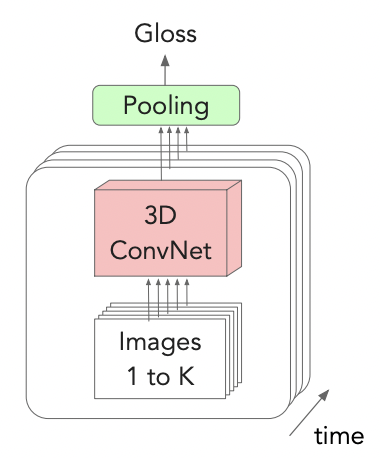
\includegraphics[width=0.4\textwidth]{assets/i3d.png}
        \caption{I3D architecture}
        \label{fig:introduction_i3d}
    \end{figure}
    \item Pose TGCN: pose based temporal graph neural network. Usually, motion is modelled using 2D joint angles.
    They encode the motion using a holistic representation of the trajectories of body keypoints. They represent
    the human body as a fully-connected graph to learn the dependencies between joints in the trajectories.
    \begin{figure}[H]
        \centering
            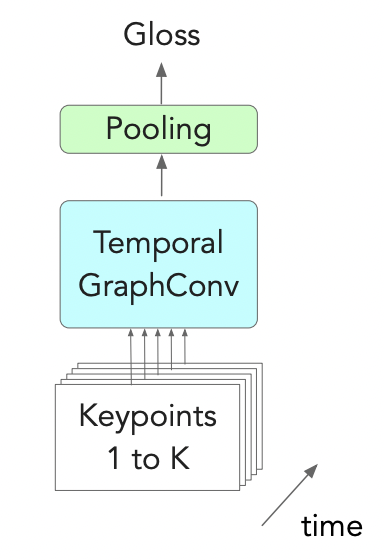
\includegraphics[width=0.4\textwidth]{assets/tgcn.png}
        \caption{TGCN architecture}
        \label{fig:introduction_tgcn}
    \end{figure}
\end{itemize}

\subparagraph{Data pre-processing} They following transformations are applied:
\begin{itemize}[noitemsep]
    \item Resize the original resolution so that the bounding-box size of the signer is 256x256 pixels.
    \item Crop a 224x224 patch from the input frame.
    \item Apply a horizontal flipping with a prob of 0.5.
\end{itemize}

\subparagraph{Implementation details and accuracy evaluation} The models are all implemented using Pytorch and the top 10 accuracy values are shown on table \ref{fig:introduction_model_accuracy_comparison}. \\
\begin{figure}[H]
    \centering
        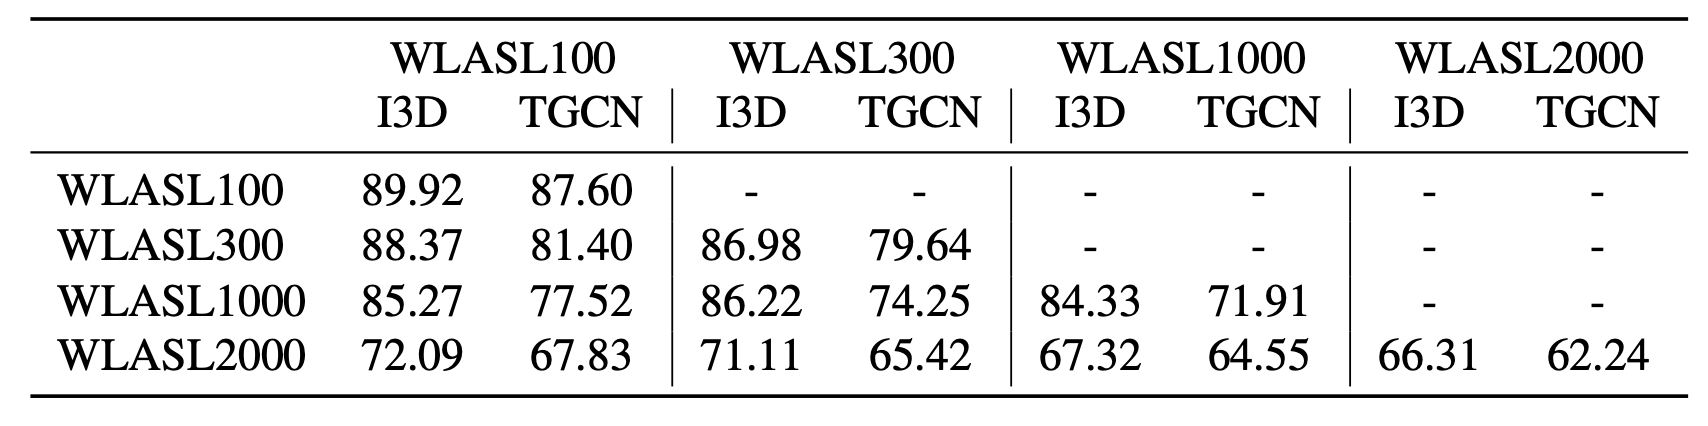
\includegraphics[width=1.0\textwidth]{assets/models_accuracy.png}
    \caption{Models' accuracy comparison}
    \label{fig:introduction_model_accuracy_comparison}
\end{figure}

I decided to use the I3D model due to its better performance.
